% Especificaciones del tamaño de letra, tamaño de hoja, márgenes, librerias, etc.
\documentclass[12pt, letterpaper]{article}
\usepackage[english]{babel}
\usepackage[utf8]{inputenc}
\usepackage[T1]{fontenc}
\usepackage{mathrsfs}
\usepackage{amsmath}
\usepackage{graphicx}
\usepackage{subcaption}
\usepackage{hyperref}
\usepackage{url}
\usepackage{amssymb}
\usepackage{float}
\usepackage[framed, numbered]{matlab-prettifier}
%\usepackage[framed, numbered, autolinebreaks, useliterate]{mcode}
\usepackage[margin=1in]{geometry}
\renewcommand{\baselinestretch}{1}

% Enlace Bibliografía
\usepackage{csquotes}
\usepackage[notes,backend=biber]{biblatex-chicago}
\addbibresource{referencias.bib}

% Titulo, autores, fecha.
\title{Tarea \#2: Respuesta Transitoria de un Sistema Dinámico}
\author{Carlos Vásquez 1155057}

% Inicio del documento
\begin{document}
\maketitle
\subsection*{Resolver el siguiente problema}
a) Encontrar la velocidad final de un auto de 1,000 kg con una fuerza de 500 N y tomando en cuenta la fricción que existe entre las llantas y el suelo de 50 $\frac{N\cdot m}{s}$. b) Encontrar el tiempo que el auto alcanzó su velocidad constante. c) Graficar la functión de $v(t)$.\\
\textbf{a) Solución}\\
Asumimos las condiciones iniciales del auto como cero. Utilizando la segunda ley de Newton podemos expresar el sistema dinámico en forma de ecuación diferencial:
\begin{equation}
	\begin{split}
		\sum F &= ma\\
		m(t) \frac{d}{dt} v(t) &= F(t) - \mu v(t)
	\end{split}
\end{equation}

Dado que la masa del sistema se mantiene constante y la fuerza de 500 N la podemos considerar como una constante aplicada al sistema cuando $t \geq 0$, nuestra ecuación diferencial se reduce a
\begin{equation}
	m \frac{d}{dt}v(t) = F\cdot \mathscr{U} (t) - \mu v(t)
\end{equation}

Aplicando la transformada de Laplace obtenemos la siguiente ecuación:
\begin{equation}
	\mathscr{L} \{ f(t) \} \Rightarrow  MsV(s) = \frac{F}{s} - \mu V(s)
\end{equation}

Despejando a $\frac{V(s)}{\mathscr{U}(s)}$ para obtener nuestra función de transferencia obtenemos:

\begin{equation}
	\boxed{\frac{V(s)}{\mathscr{U}(s)} \Rightarrow sV(s) = \frac{F}{Ms + \mu}}
\end{equation}
Sin embargo, para encontrar $v(t)$ cuando $t \rightarrow \infty$ debemos de despejar V(s) y aplicar la integral de Bromwich para obtener nuestro sistema en el dominio del tiempo.
\begin{equation}
	\begin{split}
		V(s) &= \frac{F}{Ms^2 + \mu s}\\
		\mathscr{L}^{-1} \{V(s)\} &= \frac{1}{2\pi i} \int_{\gamma - i\infty}^{\gamma + i \infty} e^{st} V(s) ds\\
	\end{split}
\end{equation}

\begin{equation}	
		\mathscr{L}^{-1} \{V(s)\} = F \left( \frac{1}{\mu} - \frac{e^{\frac{-\mu t}{M}}}{\mu}\right)
\end{equation}

Y para nuestro sistema en particular:

\begin{equation}	
		\mathscr{L}^{-1} \{V(s)\} = 500 \left( \frac{1}{50} - \frac{e^{\frac{-t}{20}}}{50}\right)
\end{equation}
Por tanto, si dejamos que $t \rightarrow \infty$, la velocidad que experimentará el automóvil será:

\begin{equation}
	\boxed{\begin{split}
		v(t \rightarrow \infty) &= 500 \left( \frac{1}{50} - 0\right)\\
		v(t \rightarrow \infty) & = \frac{500}{50} = 10\ m/s
	\end{split}}
\end{equation}\\
\textbf{b) Solución}\\
El tiempo para el cual se considera que el transitorio ha terminado es de $5\tau$ y dado que $\tau = 20$, podemos asumir que el tiempo que tarda en llegar a la velocidad final es de 100 s. Realizando el cálculo en este tiempo observamos que la velocidad para $t = 100\ s$ es bastante aproximada a 10 m/s.
\begin{equation}
	v(100\ s) = 500 \left( \frac{1}{50} - \frac{e^{\frac{-100}{20}}}{50}\right) \approx 9.9326\ m/s
\end{equation}\\
\textbf{c) Solución}\\
\lstinputlisting[style=Matlab-editor, basicstyle=\mlttfamily\scriptsize, caption={Código de la función encontrada para $v(t)$}]{./code/hw.m}

\begin{figure}[H]
	\centering
	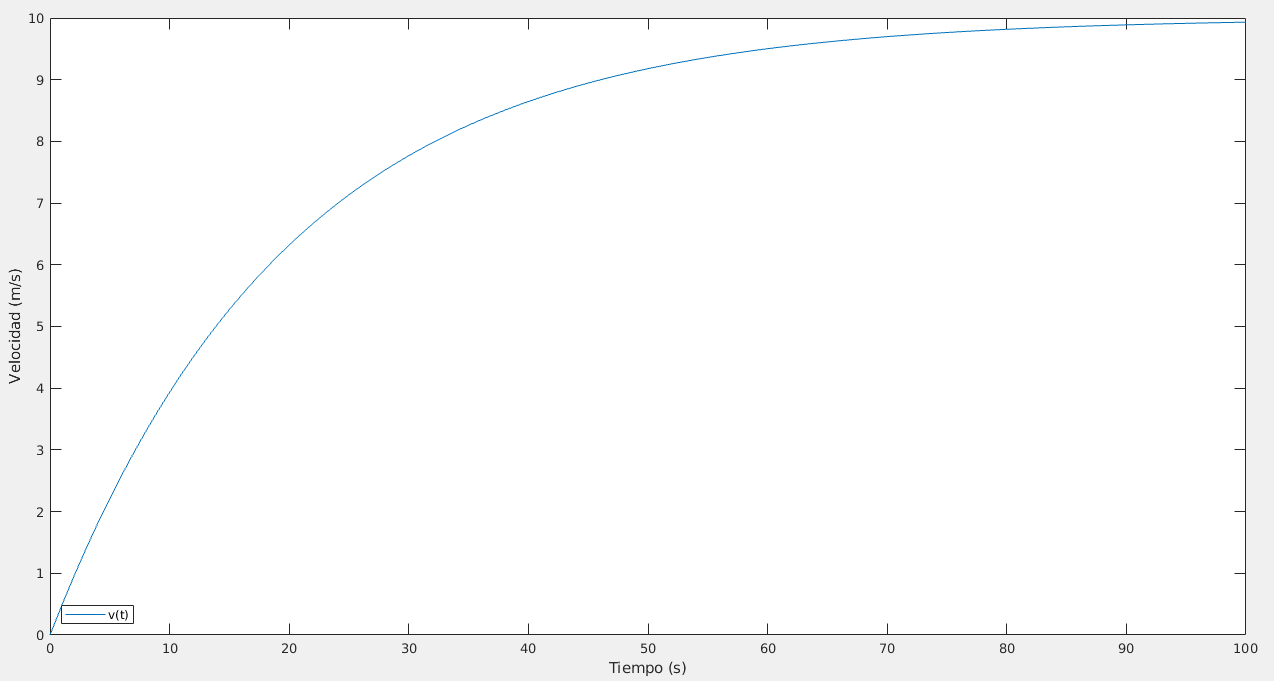
\includegraphics[width=0.75\textwidth]{plot.png}
	\caption{Gráfica de $v(t)$}
\end{figure}
%%%%% Bib
\renewcommand\refname{Referencias}
\printbibliography
\end{document}
